\section{Wprowadzenie}

Ostatnią częścią pracy inżynierskiej jest program ViuaChat - chat internetowy o funkcjonalności podobnej do IRC.
Umożliwia użytkownikom logowanie się do sieci, zakładanie pokojów tematycznych do rozmów, oraz rozmowy
''prywatne'' (tj. wyłączne dla dwóch użytkowników).

W poniższym rozdziale zdefiniowano wymagania dla czatu ViuaChat. Ich opracowanie nastąpiło na podstawie analizy otoczenia aplikacji oraz analizy potrzeb projektu w stosunku do niej. W ramach tego procesu nastąpiły:
\begin{itemize}
    \item analiza otoczenia, wraz z z klientami;
    \item wskazanie kontekstu biznesowego systemu;
    \item określenie udziałowców;
	\item wyszczególnienie i uporządkowanie zasad biznesowych, jakie zostały założone w stosunku do aplikacji;
	\item opracowanie historyjek na podstawie ustalonych zasad biznesowych.
\end{itemize}

\textbf{Uwaga:} Niniejszy rozdział nie dotyczy języka ViuAct ani jego kompilatora.

\subsection{Odbiorcy}
Rozdział został pierwotnie napisany przede wszystkim dla członków zespołu, aby ułatwić im współpracę - w szczególności wówczas, gdy funkcjonalności czatu mogły pociągać za sobą modyfikację zestawu bibliotek Viua VM bądź struktury składni projektowanego języka ViuAct.

\section{Czat w kontekście}

\subsection{Kontekst biznesowy}

Niniejszy czat stanowi część szerszego kontekstu, jakim jest potrzeba zademonstrowania działania języka ViuAct oraz całego środowiska wytwórczego powiązanego z maszyną wirtualną ViuaVM.

\begin{figure}[h]
	\centering
	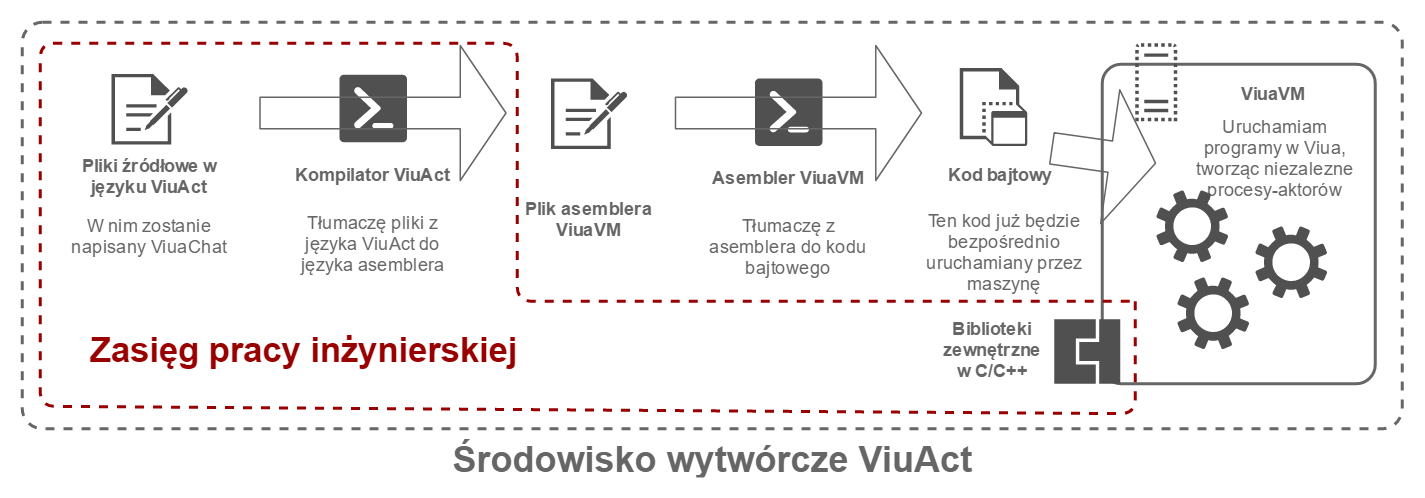
\includegraphics[width=\textwidth]{chat/fig/viuavm-env}
	\caption{Ilustracja środowiska wytwórczego wraz zasięgiem, którym są objęte prace przewidziane projektem inżynierskim}
\end{figure}

Cel demonstracyjny był pierwszym i najważniejszym, jaki przyświecał budowie
czatu. Ponadto, proces wytwórczy pozwolił przetestować wydajność całego
środowiska w jego praktycznym wymiarze. Tym samym, możliwe było poprawienie
konstrukcji kompilatora lub zastosowanych konstrukcji językowych ViuAct,
podnosząc tym samym jego użyteczność.

Wszelcy odbiorcy dla aplikacji czatu zostaną, podobnie jak sama aplikacja,
skonstruowani na cele demonstracyjne. Nie powinni oni odbiegać od modelowych
odbiorców podobnych komunikatorów, tak, aby potencjalny, poczatkujący
użytkownik środowiska ViuaVM mógł zrozumieć intencje stojące za rozwiązaniami
zastosowanymi w ViuaChat oraz przenieść je do swoich pierwszych programów.

\subsection{Udziałowcy}

Poniżej wyszczególniono udziałowców, mających wpływ na rozwój czatu.

\begin{tabular}{ | l | l | }

	\hline
	\multicolumn{2}{ | l | }{\textbf{Karta udziałowca}}  \\

	\hline
    \parbox[t]{3cm}{
    	\textbf{Identyfikator}
    } & UN-01 \\

    \hline
    \parbox[t]{3cm}{
    	\textbf{Nazwa}
    } & ViuaVM \\

    \hline
    \parbox[t]{3cm}{
    	\textbf{Opis}
    } & \parbox[t]{12cm}{
    	Maszyna wirtualna, oparta o przechowywanie danych w rejestrach zamiast
      \textit{płaskich} tablic pamięci. Stanowi ona platformę, na której musi
      zostać uruchomiony serwer czatu. Ponieważ jej największym atutem jest
      zorientowanie na kod wykonywany współbieżnie, sam serwer czatu powinien
      tę cechę wykorzystywać w maksymalnym stopniu.
    	} \\

    \hline
    \parbox[t]{3cm}{
    	\textbf{Typ}
    } & Nieożywiony, bezpośredni \\

    \hline
    \parbox[t]{3cm}{
    	\textbf{Punkt widzenia}
    } & \parbox[t]{12cm}{
    	ViuaVM jest absolutnie nieodzownym elementem projektu, a serwer czatu
      stanowi przede wszystkim dowód jej użyteczności. O ile jądro maszyny nie
      ma być poddawane już żadnym zmianom i być wykorzystane takie, jakie było
      na inicjalnym etapie pracy inżynierskiej, o tyle dopuszcza się
      poszerzanie funkcjonalności o dodatkowe biblioteki zewnętrzne.
    	} \\

    \hline
    \parbox[t]{3cm}{
    	\textbf{Ograniczenia}
    } & \parbox[t]{12cm}{
    	Maszyna wirtualna, jakkolwiek stanowi istotny czynnik dla decyzji w
      zakresie architektury czy konstrukcji oprogramowania, nie powinna mieć
      wpływu na wymagania stricte biznesowe, jest bowiem jedynie środowiskiem
      do uruchamiania współbieżnych programów, \textit{przezroczystym} dla
      końcowego użytkownika czy zleceniodawcy zrealizowanego oprogramowania.
    	} \\

    \hline
    \parbox[t]{3cm}{
    	\textbf{Wymagania}
    } & \colorbox{yellow}{...} \\

    \hline
\end{tabular}

\vspace{1em}

\begin{tabular}{ | l | l | }

	\hline
	\multicolumn{2}{ | l | }{\textbf{Karta udziałowca}}  \\

	\hline
    \parbox[t]{3cm}{
    	\textbf{Identyfikator}
    } & UO-01 \\

    \hline
    \parbox[t]{3cm}{
    	\textbf{Nazwa}
    } & Opiekun pracy inżynierskiej \\

    \hline
    \parbox[t]{3cm}{
    	\textbf{Opis}
    } & \parbox[t]{12cm}{
    	Pracownik uczelni, wyznaczony do opieki nad całym projektem inżynierskim
      - nadzorowania jego postępów, wskazywania problemów oraz sugerowania
      decyzji podwyższających walor pracy oraz szanse na jej skuteczne
      obronienie. Ma również zasadniczy wpływ na decyzję o dopuszczeniu pracy
      do recenzji.
    } \\

    \hline
    \parbox[t]{3cm}{
    	\textbf{Typ}
    } & Ożywiony, bezpośredni \\

    \hline
    \parbox[t]{3cm}{
    	\textbf{Punkt widzenia}
    } & \parbox[t]{12cm}{
    	Opiekun pracy patrzy na czat przede wszystkim przez pryzmat jego
      użyteczności jako efektownego przykładu implementacji modelu
    	aktora w praktycznym, programistycznym ujęciu. Stąd, jego uwaga skupia
      się przede wszystkim na konstrukcjach językowych, strukturach oraz
      rozwiązaniach od strony kodu źródłowego. Czat stanowi jedynie pretekst do
      przeniesienia teoretycznych, akademickich rozważań na praktyczny grunt.
    	} \\

    \hline
    \parbox[t]{3cm}{
    	\textbf{Ograniczenia}
    } & \parbox[t]{12cm}{
    	Opiekun pracy, pomimo bycia jej nadzorcą i posiadania istotnych uprawnień
      decyzyjnych w stosunku do jej dalszego rozwoju, nie ma możliwości
      bieżącego śledzenia prac oraz podejmowania decyzji w przypadku
      konkretnych problemów. Powinien zachować dystans, pozwalający na
      samodzielną realizację projektu przez zespół. Stąd, jego faktyczny udział
      ogranicza się do udzielania porad w przypadku strategicznych kierunków, w
      jakich będzie podążała grupa, a także doraźnego recenzowania ograniczonej
      puli zagadnień, wyłapanych w trakcie wspólnych spotkań.
    	} \\

    \hline
    \parbox[t]{3cm}{
    	\textbf{Wymagania}
    } & \colorbox{yellow}{...} \\

    \hline
\end{tabular}

\vspace{1em}

\begin{tabular}{ | l | l | }

	\hline
	\multicolumn{2}{ | l | }{\textbf{Karta udziałowca}}  \\

	\hline
    \parbox[t]{3cm}{
    	\textbf{Identyfikator}
    } & UO-02 \\

    \hline
    \parbox[t]{3cm}{
    	\textbf{Nazwa}
    } & \parbox[t]{12cm}{
    Członek zespołu ds. ViuAct
    } \\

    \hline
    \parbox[t]{3cm}{
    	\textbf{Opis}
    } & \parbox[t]{12cm}{
    	Student i członek zespołu, skupiający się w pierwszej kolejności nad rozwojem języka programowania ViuAct, jego kompilatora oraz
    	ewentualnego rozbudowania maszyny ViuaVM o kolejne, zewnętrzne biblioteki.
    } \\

    \hline
    \parbox[t]{3cm}{
    	\textbf{Typ}
    } & Ożywiony, bezpośredni \\

    \hline
    \parbox[t]{3cm}{
    	\textbf{Punkt widzenia}
    } & \parbox[t]{12cm}{
    	Przede wszystkim, postrzega czat jako produkt, realizowany na końcowej platformie. Stąd, musi brać udział w formułowaniu
    	wymagań związanych z ViuaVM oraz językiem ViuAct. Jego zadaniem jest doprowadzenia do zaprojektowania czatu w sposób,
    	który ukaże możliwości ViuAct jako solidnego, kompletnego rozwiązania. Przy tym, musi trzymać rękę na pulsie i reagować,
    	gdyby pojawiały się przeszkody w zaprogramowaniu czatu, wynikające z niedoskonałości środowiska wytwórczego.

    	Podczas współudziału w definiowaniu wymagań, istotny jest dla niego zakres pracy, wiążący się z
    	urzeczywistnianiem poszczególnych, proponowanych wymagań. Zbyt rozbudowany czat może opóźnić prace nad całym projektem,
    	a w efekcie - zniweczyć trud włożony w rozwój języka programowania i dedykowanego mu kompilatora.
    	} \\

    \hline
    \parbox[t]{3cm}{
    	\textbf{Ograniczenia}
    } & \parbox[t]{12cm}{
    	Jego udział w pracach nad czatem jest z gruntu nieograniczony. Jednakże, decydując się na podział odpowiedzialności
    	podyktowany zespołowym charakterem projektu oraz własnymi ograniczeniami czasowymi, zrezygnował z decydowania o biznesowej
    	części wymagań, faktycznie pozostając w roli konsultanta.

    	} \\

    \hline
    \parbox[t]{3cm}{
    	\textbf{Wymagania}
    } & \colorbox{yellow}{...} \\

    \hline
\end{tabular}

\vspace{1em}

\begin{tabular}{ | l | l | }

	\hline
	\multicolumn{2}{ | l | }{\textbf{Karta udziałowca}}  \\

	\hline
    \parbox[t]{3cm}{
    	\textbf{Identyfikator}
    } & UO-03 \\

    \hline
    \parbox[t]{3cm}{
    	\textbf{Nazwa}
    } & \parbox[t]{12cm}{
    Członek zespołu ds. Czatu
    } \\

    \hline
    \parbox[t]{3cm}{
    	\textbf{Opis}
    } & \parbox[t]{12cm}{
    	Student i członek zespołu, odpowiedzialny za prace nad czatem
    } \\

    \hline
    \parbox[t]{3cm}{
    	\textbf{Typ}
    } & Ożywiony, bezpośredni \\

    \hline
    \parbox[t]{3cm}{
    	\textbf{Punkt widzenia}
    } & \parbox[t]{12cm}{
    	Czat stanowi dla niego, obok dokumentacji, najistotniejszą część przedsięwzięcia. Musi z jednej strony nauczyć się poruszać
    	w nowym, dynamicznie zmieniającym się środowisku programistycznym, a z drugiej strony - zrealizować przy jego użyciu serwer
    	czatu, który pokaże jego możliwości i zastosowania innym nowicjuszom.

    	Podczas współudziału w definiowaniu wymagań, istotny jest dla niego zakres końcowych funkcjonalności czatu. Nie może być zbyt
    	wąski. Z drugiej strony, konstrukcja programu powinna pozostać prosta i przejrzysta. Przykładowy kod nie powinien odstraszać
    	potencjalnego programisty, dla którego cała koncepcja ViuaVM oraz modelu aktorów może wydawać się na pierwszy rzut oka nieco egzotyczna.
    	} \\

    \hline
    \parbox[t]{3cm}{
    	\textbf{Ograniczenia}
    } & \parbox[t]{12cm}{
    	Nie ma w zasadzie organizacyjnych czy kompetencyjnych ograniczeń dla formułowania wymagań. Nie oznacza to jednak, że może
    	definiować wymagań w oderwaniu od pozostałych udziałowców (ich role i punkty widzenia opisano wcześniej).
    	} \\

    \hline
    \parbox[t]{3cm}{
    	\textbf{Wymagania}
    } & \colorbox{yellow}{...} \\

    \hline
\end{tabular}

\subsection{Charakterystyka użytkowników}

Na etapie analizy kontekstu, w którym ma zostać zaprojektowany i zrealizowany czat, zadecydowano o zaprojektowaniu następujących,
modelowych użytkowników docelowego oprogramowania:

\begin{enumerate}

	\item \textbf{Użytkownik tymczasowy.} Typ użytkownika, którego konto jest tworzone podczas połączenia z serwerem czatu oraz
		niszczone po jego zakończeniu. Podczas łączenia z czatem, nie będzie musiał się autoryzować przy użyciu hasła, a deklarować
		tylko unikalną nazwę, nie powtarzającą się z nazwą innego użytkownika, posiadającego konto na danym serwerze czatu.

	\item \textbf{Użytkownik stały.} Typ użytkownika, którego W
		zamierzeniu, adresatami takiego rozwiązania mają być stali bywalcy serwera, którzy chcą mieć zarezerwowaną określoną nazwę
		dla siebie i uniknąć ewentualnego podszywania się. Stąd

	\item \textbf{Administrator.} To użytkownik, który jest dodatkowo wyróżniony i posiada uprawienia do szeroko pojętego
		zarządzania serwerem (w tym - pozostałymi użytkownikami). Konto administratora jest utrzymywane przez serwer pomiędzy połączeniami do czatu. Każdorazowo, przed rozpoczęciem sesji połączenia z serwerem, muszą się dodatkowo autoryzować przy użyciu hasła. Równocześnie, ich nazwa jest zarezerwowana wyłącznie do jego użytku oraz niedostępna
		dla użytkowników tymczasowych.Nie wyróżnia się wśród administratorów żadnych dodatkowych, szczególnych
		ról (np. superadministrator, właściciel).

\end{enumerate}

Poza wspomnianymi różnicami, wszyscy użytkownicy po rozpoczęciu sesji połączenia mają prawo do dołączania do pokojów oraz wysyłania sobie
nawzajem wiadomości prywatnych. Łącznie, pula użytkowników przebywających na serwerze czatu w jednym momencie nie powinna przekraczać 320,
zaś w jednym pokoju - nie więcej niż 32. W związku z tym można przyjąć, że czat jest przeznaczony dla niewielkich społeczności, np.
szkolnych, uczelnianych czy hobbystycznych.

\subsection{Istniejąca infrastruktura}
\label{existing-infr}
\begin{itemize}
	\item \textbf{Komputer A}
	\begin{itemize}
		\item komputer przenośny z procesorem Intel Core i5 oraz systemem operacyjnym Windows 10
		\item XAMPP 7.2.7, obejmujący serwer Apache 2.4 oraz interpreter języka PHP w wersji 7.2.7.
    \item oprogramowanie VirtualBox z uruchomioną maszyną wirtualną z systemem
    operacyjnym Linux Mint 19 ,,Tara''.
	\end{itemize}

	\item \textbf{Komputer B}
	\begin{itemize}
		\item komputer przenośny, na którym zainstalowano system operacyjny Linux Mint 19 ,,Tara''
		\item GNU Compiler Collection 8.2
		\item wirtualna maszyna Viua VM w wersji 0.9.0
		\item \textit{należy doinstalować serwer Nginx, odpowiedzialny za wysłanie frontendu do
		użytkownika łączącego się z czatem oraz za handshake Websocketu}
	\end{itemize}

	\item \textit{\textbf{Do uzupełnienia}
	\begin{itemize}
		\item Kolejne urządzenie końcowe (trzecie), dzięki któremu będzie można symulować połączenie kolejnej
		osoby do usługi czatu
	\end{itemize}}

\end{itemize}

\section{Zasady biznesowe}

Zidentyfikowane zasady pogrupowano w 3 kategorie, biorąc pod uwagę podstawowe bloki funkcjonalności. Przydzielenie
do kategorii jest sygnalizowanie literą alfabetu, będącą prefiksem identyfikatora danej zasady. Numeracja identyfikatorów może być nieciągła, gdyż
część z wymagań została usunięta w trakcie prac nad dokumentacją.

Dokonano
również priorytetyzacji zasad biznesowych według klasycznej skali ,,MoSCoW":

\begin{itemize}
	\item \textbf{,,M''} (z ang. \textit{must}) - zasady, których spełnienie jest niezbędne dla realizacji systemu
	\item \textbf{,,S''} (z ang. \textit{should}) - są to zasady o wysokim priorytecie, które powinny;
	zostać spełnione, o ile tylko jest to możliwe;
	\item \textbf{,,C''} (z ang. \textit{could}) - dobrze byłoby zrealizować takie wymagania, ale zależy to od czasu
	i zasobów, jakie pozostaną do dyspozycji po ukończeniu zadań ,,M" i ,,C";
	\item \textbf{,,W''} (z ang. \textit{won't}) - takie wymagania, po dyskusji, zostały wycofane dalszej realizacji.
\end{itemize}

\newpage

\subsection{System użytkowników [ZU]}

\leavevmode\hbox{}

  \begin{tabular}{ | l | l | l | }
	\hline
    \textbf{ID} & \parbox[t]{12cm}{\strut
    	\textbf{Zasada biznesowa}
    \strut} & \textbf{Priorytet} \\

    \hline
      \parbox[t]{1.2cm}{
        ZU-01

      } & \parbox[t]{12.1cm}{\strut
        Podczas wejścia na czat, użytkownikowi pokazuje się monit z polem do wpisania nazwy użytkownika.
      \strut} & \parbox{1.8cm}{
        M

      } \\

    \hline
      \parbox[t]{1.2cm}{
        ZU-02

      } & \parbox[t]{12.1cm}{\strut
        Użytkownicy bez stałego konta podczas logowania podają tylko nazwę użytkownika, pole hasła pozostaje puste.

      \strut} & \parbox{1.8cm}{
        M

      } \\

    \hline
      \parbox[t]{1.2cm}{
        ZU-03

      } & \parbox[t]{12.1cm}{\strut
        Nazwa użytkownika to ciąg od 3 do 32 alfanumerycznych znaków.

      \strut} & \parbox{1.8cm}{
        M

      } \\

    \hline
      \parbox[t]{1.2cm}{
        ZU-04
      } & \parbox[t]{12.1cm}{\strut
      Można rozpocząć sesję jako użytkownik, pod warunkiem, że zadeklarowana nazwa nie będzie powtarzać się z nazwami ju  ż
      zalogowanych użytkowników.
    \strut} & \parbox{1.8cm}{
      M

    } \\

    \hline
      \parbox[t]{1.2cm}{
        ZU-05

      } & \parbox[t]{12.1cm}{\strut
        Monit podczas wejścia na czat jest wyposażony w pole do wpisania hasła (nieobowiązkowe).

      \strut} & \parbox{1.8cm}{
        S

      } \\

    \hline
      \parbox[t]{1.2cm}{
        ZU-06

      } & \parbox[t]{12.1cm}{\strut
        Administrator podczas logowania podają nazwę i odpowiadające mu hasło.

      \strut} & \parbox{1.8cm}{
        S

      } \\

    \hline
      \parbox[t]{1.2cm}{
        ZU-07

      } & \parbox[t]{12.1cm}{\strut
        Konta administratorów są utrzymywane na serwerze w postaci par wartości: nazwa użytkownika i hasło.

      \strut} & \parbox{1.8cm}{
        S

      } \\

    \hline
      \parbox[t]{1.2cm}{
        ZU-08
      } & \parbox[t]{12.1cm}{\strut
      Nie można rozpocząć sesji użytkownika o nazwie, która pasuje do istniejącego konta, jeżeli nie zostanie podan e
      prawidłowe hasło (nie można podszywać się pod nazwy administratorów).
    \strut} & \parbox{1.8cm}{
      S

    } \\

    \hline
      \parbox[t]{1.2cm}{
        ZU-09
      } & \parbox[t]{12.1cm}{\strut
      Można rozpocząć sesję jako użytkownik bez podawania hasła, pod warunkiem, że zadeklarowana nazwa nie będzie powtarza  ć
      się z nazwami kont administratorów i już zalogowanych użytkowników tymczasowych.
    \strut} & \parbox{1.8cm}{
      S

    } \\

    \hline
      \parbox[t]{1.2cm}{
        ZU-10

      } & \parbox[t]{12.1cm}{\strut
      W okienkach czatu, loginy administratorów są pogrubione i pokolorowane na czerwono.

        \strut} & \parbox{1.8cm}{
          S

        } \\

    \hline
      \parbox[t]{1.2cm}{
        ZU-11

      } & \parbox[t]{12.1cm}{\strut
        Administratorzy mają prawo przeglądać nazwy pokojów na serwerze.

      \strut} & \parbox{1.8cm}{
        M

      } \\

    \hline
      \parbox[t]{1.2cm}{
        ZU-12

      } & \parbox[t]{12.1cm}{\strut
        Administratorzy mają prawo tworzyć i usuwać pokoje.

      \strut} & \parbox{1.8cm}{
        S

      } \\

    \hline
      \parbox[t]{1.2cm}{
        ZU-14

      } & \parbox[t]{12.1cm}{\strut
        Administratorzy mają prawo wyrzucać użytkowników z pokojów.

      \strut} & \parbox{1.8cm}{
        C

      } \\

    \hline
      \parbox[t]{1.2cm}{
        ZU-15

      } & \parbox[t]{12.1cm}{\strut
        Administratorzy mają prawo wyrzucać użytkowników z serwera.

      \strut} & \parbox{1.8cm}{
        C

      } \\

    \hline
      \parbox[t]{1.2cm}{
        ZU-16

      } & \parbox[t]{12.1cm}{\strut
        Administratorzy mają prawo przeglądać nazwy i poziomy uprawnień użytkowników.

      \strut} & \parbox{1.8cm}{
        M

      } \\

    \hline
      \parbox[t]{1.2cm}{
        ZU-18

      } & \parbox[t]{12.1cm}{\strut
        Administratorzy mają prawo zmieniać swoje hasła użytkowników.

      \strut} & \parbox{1.8cm}{
        C

      } \\

    \hline
  \end{tabular}

\newpage

\subsection{Pokoje [ZP]}

\leavevmode\hbox{}

  \begin{tabular}{ | l | l | l | }
	\hline
    \textbf{ID} & \parbox[t]{12cm}{\strut
    	\textbf{Zasada biznesowa}
    } & \textbf{Priorytet} \\

    \hline
    \parbox[t]{1.2cm}{
      ZP-01

    } & \parbox[t]{12.1cm}{\strut
      Pokoje to właściwe czaty – tam użytkownicy mogą wejść i pisać do siebie nazwajem

    \strut} & \parbox[t]{1.8cm}{
      M

    } \\

    \hline
    \parbox[t]{1.2cm}{
      ZP-02

    } & \parbox[t]{12.1cm}{\strut
      Każdy pokój ma unikalną nazwę będącą ciągiem alfanumerycznym od 3 do 32 znaków

    \strut} & \parbox[t]{1.8cm}{
      M

    } \\

    \hline
    \parbox[t]{1.2cm}{
      ZP-03

    } & \parbox[t]{12.1cm}{\strut
      Lista pokojów jest widoczna dla każdego użytkownika po zalogowaniu się do serwera czatu

    \strut} & \parbox[t]{1.8cm}{
      M

    } \\

    \hline
    \parbox[t]{1.2cm}{
      ZP-04

    } & \parbox[t]{12.1cm}{\strut
      Użytkownik może być równocześnie wpięty do jednego pokoju

    \strut} & \parbox[t]{1.8cm}{
      M

    } \\

    \hline
    \parbox[t]{1.2cm}{
      ZP-05

    } & \parbox[t]{12.1cm}{\strut
      Wiadomość wysłana w pokoju jest widoczna w oknie pokoju dla wszystkich użytkowników podpiętych do tego pokoju

    \strut} & \parbox[t]{1.8cm}{
      M

    } \\

    \hline
    \parbox[t]{1.2cm}{
      ZP-06

    } & \parbox[t]{12.1cm}{\strut
      Użytkownik może się samodzielnie wypiąć z pokoju, do którego jest wpięty

    \strut} & \parbox[t]{1.8cm}{
      S

    } \\

    \hline
    \parbox[t]{1.2cm}{
      ZP-07

    } & \parbox[t]{12.1cm}{\strut
      Pokój może mieć ustanowione hasło, które użytkownik musi wpisać przed podpięciem się do niego

    \strut} & \parbox[t]{1.8cm}{
      C

    } \\

    \hline
    \parbox[t]{1.2cm}{
      ZP-08

    } & \parbox[t]{12.1cm}{\strut
      Nowo wpięty użytkownik widzi 10 najnowszych wiadomości,
      które zostały wysłane do pokoju tuż przed wpięciem

    \strut} & \parbox[t]{1.8cm}{
      S

    } \\

    \hline
    \parbox[t]{1.2cm}{
      ZP-09

    } & \parbox[t]{12.1cm}{\strut
      Serwer czatu automatycznie wysyła do pokoju wiadomości,
      zawierające powiadomienia o wydarzeniach związanych z
      pokojem, tzw. wiadomości systemowe

    \strut} & \parbox[t]{1.8cm}{
      S

    } \\

    \hline
    \parbox[t]{1.2cm}{
      ZP-10

    } & \parbox[t]{12.1cm}{\strut
      Wiadomości systemowe są niepodpisane przez
      żadnego użytkownika i zapisane kursywą

    \strut} & \parbox[t]{1.8cm}{
      C

    } \\

   	\hline
    \parbox[t]{1.2cm}{
      ZP-11

    } & \parbox[t]{12.1cm}{\strut
      Wiadomość systemowa zostaje wysłana podczas wpięcia się
      nowego użytkownika do pokoju

    \strut} & \parbox[t]{1.8cm}{
      S

    } \\

   	\hline
    \parbox[t]{1.2cm}{
      ZP-12

    } & \parbox[t]{12.1cm}{\strut
      Wiadomość systemowa zostaje wysłana podczas wypięcia
      użytkownika z pokoju

    \strut} & \parbox[t]{1.8cm}{
      S

    } \\

   	\hline
    \parbox[t]{1.2cm}{
      ZP-13

    } & \parbox[t]{12.1cm}{\strut
      Wiadomość systemowa zostaje wysłana, gdy użytkownik
      wpięty do pokoju traci połączenie z serwerem czatu

    \strut} & \parbox[t]{1.8cm}{
      S

    } \\

   	\hline
    \parbox[t]{1.2cm}{
      ZP-14

    } & \parbox[t]{12.1cm}{\strut
      Wiadomość systemowa zostaje wysłana, gdy użytkownik
      zostaje wyrzucony z pokoju

    \strut} & \parbox[t]{1.8cm}{
      S

    } \\

    \hline

  \end{tabular}

\newpage

\subsection{Prywatne wiadomości [ZW]}

\leavevmode\hbox{}

  \begin{tabular}{ | l | l | l | }
  	\hline
    \textbf{ID} & \parbox[t]{12cm}{
    	\textbf{Zasada biznesowa}
    } & \textbf{Priorytet} \\

    \hline
    \parbox{1.2cm}{
      ZW-01

    } & \parbox[t]{12.1cm}{\strut
      Wiadomości prywatne to wiadomości, które są wysyłane do
      konkretnego odbiorcy, innego niż nadawca. Są one widoczne
      wyłącznie dla nadawcy i odbiorcy takiej wiadomości

    \strut} & \parbox{1.8cm}{
      M

    } \\

    \hline
    \parbox{1.2cm}{
      ZW-06

    } & \parbox[t]{12.1cm}{\strut
      Użytkownik dysponuje dedykowanym oknem, w którym widzi wiadomości prywatne.

    \strut} & \parbox{1.8cm}{
      M

    } \\

    \hline
    \parbox{1.2cm}{
      ZW-07

    } & \parbox[t]{12.1cm}{\strut
      Z okna wiadomości prywatnych można odbierać i wysyłać wyłącznie
      wiadomości prywatne, których nadawcą/odbiorcą jest wybrany
      użytkownik

    \strut} & \parbox{1.8cm}{
      M

    } \\

    \hline
    \parbox{1.2cm}{
      ZW-08

    } & \parbox[t]{12.1cm}{\strut
      W oknie wiadomości prywatnych można przeglądać wiadomości wysłane do i odebrane od jednego, wybranego użytkownika.


    \strut} & \parbox{1.8cm}{
      S

    } \\

    \hline
    \parbox{1.2cm}{
      ZW-09

    } & \parbox[t]{12.1cm}{\strut
      W oknie wiadomości prywatnych można wysyłać wiadomości
      wyłącznie do nadawcy, którego wiadomości są w danym momencie
      pokazywane.

    \strut} & \parbox{1.8cm}{
      S

    } \\

    \hline
    \parbox{1.2cm}{
      ZW-10

    } & \parbox[t]{12.1cm}{\strut
      Wiadomości prywatne są utrzymywane dopóki nadawca i odbiorca mają aktywną
      sesję na serwerze.

    \strut} & \parbox{1.8cm}{
      S

    } \\

    \hline
    \parbox{1.2cm}{
      ZW-11

    } & \parbox[t]{12.1cm}{\strut
      Dla każdej pary użytkowników, na serwerze jest
      gromadzone co najwyżej 100 wiadomości prywatnych.

    \strut} & \parbox{1.8cm}{
      S

    } \\
    \hline
  \end{tabular}

\newpage

\section{Wymagania}
\label{program_viuachat_wymagania}

\subsection{Wymagania funkcjonalne}

Ponieważ obraną metodologią wytwarzania aplikacji jest \textit{mini-Scrum}, należący do kategorii metodyk zwinnych, wymagania funkcjonalne ujęto w formie historyjek (\textit{user stories}).

\vspace{1em}

\begin{tabular}{ | l | l | }
	\hline
		\textbf{Identyfikator} &
		WF-01
		\\

	\hline
		\textbf{Treść} & \parbox[t]{11.5cm}{\strut
			Jako użytkownik serwera czatu, chcę się do niego zalogować, aby zobaczyć listę pokojów dyskusyjnych.
		\strut}\\

	\hline
		\parbox[t]{4cm}{\textbf{Powiązane zasady biznesowe}} & \parbox[t]{11.5cm}{\strut
			ZU-01 Podczas wejścia na czat, użytkownikowi pokazuje się monit z polem do wpisania nazwy użytkownika. \\
			ZP-03 Lista pokojów jest widoczna dla każdego użytkownika
			po zalogowaniu się do serwera czatu
		\strut}\\

	\hline
		\parbox[t]{4cm}{\textbf{Kryteria akceptacji}} & \parbox[t]{11.5cm}{\strut
			\begin{enumreq}
				\item Po wejściu na czat bez rozpoczętej sesji, pokazuje się monit o podanie nazwy użytkownika.
				\item Po wpisaniu nazwy użytkownika i zatwierdzeniu, użytkownik rozpocznie sesję na serwerze czatu.
				\item Tuż po rozpoczęciu sesji czatu, użytkownik zobaczy listę pokojów.
			\end{enumreq}
			\strut}
		\\

	\hline
\end{tabular}

\vspace{1em}

\begin{tabular}{ | l | l | }
	\hline
		\textbf{Identyfikator} &
		WF-02
		\\

	\hline
		\textbf{Treść} & \parbox[t]{11.5cm}{\strut
			Jako użytkownik serwera czatu, chcę wpiąć się do pokoju,
			aby wziąć udział w dyskusji.
		\strut}\\

	\hline
		\parbox[t]{4cm}{\textbf{Powiązane zasady biznesowe}} & \parbox[t]{11.5cm}{\strut
			ZP-01 Pokoje to właściwe czaty - tam użytkownicy mogą
			wejść i pisać do siebie nawzajem
		\strut}\\

	\hline
		\parbox[t]{4cm}{\textbf{Kryteria akceptacji}} & \parbox[t]{11.5cm}{\strut
			\begin{enumreq}
				\item Użytkownik, który ma otwartą sesję
				połączenia z serwerem czatu i nie jest wpięty
				do żadnego pokoju, zobaczy listę pokojów.
				\item Użytkownik, po kilknięciu w liście pokojów
				na nazwę pokoju, zostanie do niego podpięty
				\item Użytkownik po wpięciu się do pokoju zobaczy
				okno pokoju
				\item Użytkownik, który ma otwartą sesję
				połączenia z serwerem i jest wpięty do pokoju,
				po odświeżeniu przeglądarki zobaczy okno pokoju,
				do którego jest wpięty
			\end{enumreq}
			\strut}
		\\

	\hline
\end{tabular}

\vspace{1em}

\begin{tabular}{ | l | l | }
	\hline
		\textbf{Identyfikator} &
		WF-03
		\\

	\hline
		\textbf{Treść} & \parbox[t]{11.5cm}{\strut
			Jako użytkownik serwera czatu, chcę po wpięciu
			do pokoju zobaczyć ostatnie wiadomości wysłane
			przed moim dołączeniem, aby dowiedzieć się, co
			tam się obecnie dzieje.
		\strut}\\

	\hline
		\parbox[t]{4cm}{\textbf{Powiązane zasady biznesowe}} & \parbox[t]{11.5cm}{\strut
			ZP-08 Nowo wpięty użytkownik widzi 10 najnowszych
			wiadomości, które zostały wysłane do pokoju tuż
			przed wpięciem
		\strut}\\

	\hline
		\parbox[t]{4cm}{\textbf{Kryteria akceptacji}} & \parbox[t]{11.5cm}{\strut
			\begin{enumreq}
				\item Użytkownik po wpięciu się do pokoju zobaczy
				10 najnowszych wiadomości wysłanych do pokoju
				przed jego dołączeniem (lub mniej, jeżeli
				dotychczas nie wysłano do pokoju co najmniej
				10 wiadomości)
			\end{enumreq}
			\strut}
		\\

	\hline
\end{tabular}

\vspace{1em}

\begin{tabular}{ | l | l | }
	\hline
		\textbf{Identyfikator} &
		WF-04
		\\

	\hline
		\textbf{Treść} & \parbox[t]{11.5cm}{\strut
			Jako użytkownik serwera czatu, chcę chcę wysłać
			wiadomość do pokoju w który jestem wpięty, aby
			zobaczyli ją inni uczestnicy dyskusji.
		\strut}\\

	\hline
		\parbox[t]{4cm}{\textbf{Powiązane zasady biznesowe}} & \parbox[t]{11.5cm}{\strut
			ZP-01 Pokoje to właściwe czaty - tam użytkownicy mogą
			wejść i pisać do siebie nawzajem
		\strut}\\

	\hline
		\parbox[t]{4cm}{\textbf{Kryteria akceptacji}} & \parbox[t]{11.5cm}{\strut
			\begin{enumreq}
				\item Użytkownik wpisze tekst wiadomości w polu
				tekstowym u dołu czatu
				\item Wiadomość wpisana w polu tekstowym zostanie
				wysłana po wciśnięciu klawisza ,,Enter'', gdy aktywne
				będzie pole tekstowe
				\item Wiadomość wpisana w polu tekstowym zostanie
				wysłana po naciśnięciu przycisku ,,Wyślij'',
				widocznego obok pola tekstowego
				\item Po wysłaniu wiadomości, pole tekstowe zostanie
				wyczyszczone (niezależnie od tego czy wiadomość
				zostanie doręczona)
				\item Wiadomość wysłana do pokoju jest pokazywana
				wszystkim użytkownikom podpiętym do czatu u dołu
				strony
				\item Nowa wiadomość jest pokazywana wraz z nazwą
				użytkownika wysyłającego u dołu konwersacji
			\end{enumreq}
			\strut}
		\\

	\hline
\end{tabular}

\vspace{1em}

\begin{tabular}{ | l | l | }
	\hline
		\textbf{Identyfikator} &
		WF-05
		\\

	\hline
		\textbf{Treść} & \parbox[t]{11.5cm}{\strut
			Jako użytkownik serwera czatu, chcę chcę zobaczyć
			powiadomienie o wpięciu się nowego użytkownika do
			pokoju w którym sam jestem obecnie wpięty, aby powitać
			nowego dyskutanta
		\strut}\\

	\hline
		\parbox[t]{4cm}{\textbf{Powiązane zasady biznesowe}} & \parbox[t]{11.5cm}{\strut
			ZP-09 Serwer czatu automatycznie wysyła do pokoju
			wiadomości, zawierające powiadomienia o wydarzeniach
			związanych z pokojem, tzw. wiadomości systemowe \\
			ZP-11 Wiadomość systemowa zostaje wysłana podczas
			wpięcia się nowego użytkownika do pokoju
		\strut}\\

	\hline
		\parbox[t]{4cm}{\textbf{Kryteria akceptacji}} & \parbox[t]{11.5cm}{\strut
			\begin{enumreq}
				\item Niezwłocznie po wpięciu się użytkownika do
				pokoju, serwer wyśle wiadomość systemową o treści
				,,Użytkownik ... dołączył do pokoju'', widoczną
				dla wszystkich użytkowników wpiętych do tego pokoju
			\end{enumreq}
			\strut}
		\\

	\hline
\end{tabular}

\vspace{1em}

\begin{tabular}{ | l | l | }
	\hline
		\textbf{Identyfikator} &
		WF-06
		\\

	\hline
		\textbf{Treść} & \parbox[t]{11.5cm}{\strut
			Jako użytkownik serwera czatu, chcę zobaczyć
			powiadomienie o opuszczeniu pokoju przez użytkownika,
			aby łatwo zorientować się, że nie bierze już udziału
			w dyskusji.
		\strut}\\

	\hline
		\parbox[t]{4cm}{\textbf{Powiązane zasady biznesowe}} & \parbox[t]{11.5cm}{\strut
			ZP-09 Serwer czatu automatycznie wysyła do pokoju
			wiadomości, zawierające powiadomienia o wydarzeniach
			związanych z pokojem, tzw. wiadomości systemowe \\
			ZP-12 Wiadomość systemowa zostaje wysłana podczas
			wpięcia wypięcia użytkownika z pokoju \\
			ZP-13 Wiadomość systemowa zostaje wysłana, gdy użytkownik
			wpięty do pokoju traci połączenie z serwerem \\
			ZP-14 Wiadomość systemowa zostaje wysłana, gdy użytkownik
			zostaje wyrzucony z pokoju

		\strut}\\

	\hline
		\parbox[t]{4cm}{\textbf{Kryteria akceptacji}} & \parbox[t]{11.5cm}{\strut
			\begin{enumreq}
				\item Niezwłocznie po wypięciu się użytkownika z
				pokoju, serwer wyśle wiadomość systemową, widoczną
				dla wszystkich użytkowników wpiętych do tego pokoju,
				o treści:
				\begin{enumerate}
					\item ,,Użytkownik ... opuścił pokój'', gdy
					użytkownik samodzielnie wypiął się z pokoju
					\item ,,Użytkownik ... stracił połączenie'',
					gdy użytkownik został wypięty z pokoju na skutek
					przerwania sesji z uwagi na zerwanie połączenia
					\item ,,Użytkownik ... został wyrzucony'', gdy
					użytkownik został wypięty wskutek interwencji
					administratora
				\end{enumerate}
			\end{enumreq}
			\strut}
		\\

	\hline
\end{tabular}

\vspace{1em}

\begin{tabular}{ | l | l | }
	\hline
		\textbf{Identyfikator} &
		WF-07
		\\

	\hline
		\textbf{Treść} & \parbox[t]{11.5cm}{\strut
			Jako użytkownik serwera czatu, chcę odpiąć się od pokoju,
			aby wpiąć się do innego pokoju.
		\strut}\\

	\hline
		\parbox[t]{4cm}{\textbf{Powiązane zasady biznesowe}} & \parbox[t]{11.5cm}{\strut
			ZP-06 Użytkownik może się samodzielnie wypiąć z pokoju,
			do którego jest wpięty

		\strut}\\

	\hline
		\parbox[t]{4cm}{\textbf{Kryteria akceptacji}} & \parbox[t]{11.5cm}{\strut
			\begin{enumreq}
				\item W oknie pokoju użytkownik zobaczy przycisk
				lub link ,,Opuść pokój''.
				\item Po kliknięciu w ,,Opuść pokój'', użytkownik
				zobaczy listę pokojów.
			\end{enumreq}
			\strut}
		\\

	\hline
\end{tabular}

\vspace{1em}

\begin{tabular}{ | l | l | }
	\hline
		\textbf{Identyfikator} &
		WF-08
		\\

	\hline
		\textbf{Treść} & \parbox[t]{11.5cm}{\strut
			Jako użytkownik serwera czatu, chcę zobaczyć
			okno wiadomości prywatnych, aby odczytać wiadomości,
			które wysłano specjalnie do mnie.
		\strut}\\

	\hline
		\parbox[t]{4cm}{\textbf{Powiązane zasady biznesowe}} & \parbox[t]{11.5cm}{\strut
			ZW-01 Wiadomości prywatne to wiadomości, które są
			wysyłane do konkretnego odbiorcy, innego niż
			nadawca... \\
			ZW-06 Użytkownik dysponuje dodatkowym oknem, na którym
			widzi wiadomości prywatne. \\
			ZW-07 Z okna wiadomości prywatnych można odbierać i
			wysyłać wyłącznie wiadomości prywatne, których
			nadawcą / odbiorcą jest wybrany użytkownik. \\
		\strut}\\

	\hline
		\parbox[t]{4cm}{\textbf{Kryteria akceptacji}} & \parbox[t]{11.5cm}{\strut
			\begin{enumreq}
				\item Po kliknięciu w link ,,PW'', użytkownik
				zobaczy okno prywatnych wiadomości
				\item W oknie wiadomości prywatnych, użytkownik
				zobaczy listę użytkowników, od których otrzymał
				wiadomości prywatne.
				\item Po kliknięciu w link z nazwą użytkownika,
				użytkownik zobaczy prywatne wiadomości, których
				nadawcą i odbiorcą jest wskazana osoba.
			\end{enumreq}
			\strut}
		\\

	\hline
\end{tabular}

\vspace{1em}

\begin{tabular}{ | l | l | }
	\hline
		\textbf{Identyfikator} &
		WF-09
		\\

	\hline
		\textbf{Treść} & \parbox[t]{11.5cm}{\strut
			Jako użytkownik serwera czatu, chcę wysłać
			wiadomość prywatną do jednego użytkownika, aby
			prowadzić z nim ciągłą konwersację.
		\strut}\\

	\hline
		\parbox[t]{4cm}{\textbf{Powiązane zasady biznesowe}} & \parbox[t]{11.5cm}{\strut


		\strut}\\

	\hline
		\parbox[t]{4cm}{\textbf{Kryteria akceptacji}} & \parbox[t]{11.5cm}{\strut
			\begin{enumreq}
				\item Użytkownik wpisze tekst wiadomości w polu
				tekstowym u dołu okna wiadomości prywatnych
				\item Wiadomość wpisana w polu tekstowym zostanie
				wysłana po wciśnięciu klawisza ,,Enter'', gdy
				aktywne
				będzie pole tekstowe
				\item Wiadomość wpisana w polu tekstowym zostanie
				wysłana po naciśnięciu przycisku ,,Wyślij'',
				widocznego obok pola tekstowego
				\item Po wysłaniu wiadomości, pole tekstowe zostanie
				wyczyszczone (niezależnie od tego czy wiadomość
				zostanie doręczona)
				\item Wiadomość wysłana w oknie zostanie pokazana
				tylko użytkownikowi, z którym trwa otwarta
				konwersacja
				\item Nowa wiadomość jest pokazywana wraz z nazwą
				użytkownika wysyłającego u dołu konwersacji
			\end{enumreq}
			\strut}
		\\

	\hline
\end{tabular}

\vspace{1em}

\begin{tabular}{ | l | l | }
	\hline
		\textbf{Identyfikator} &
		WF-11
		\\

	\hline
		\textbf{Treść} & \parbox[t]{11.5cm}{\strut
			Jako użytkownik serwera czatu, chcę wysłać wiadomość
			prywatną do innego użytkownika, z którym wcześniej nie
			wymieniałem takich wiadomości, aby rozpocząć z nim
			prywatną konwersację.
		\strut}\\

	\hline
		\parbox[t]{4cm}{\textbf{Powiązane zasady biznesowe}} & \parbox[t]{11.5cm}{\strut
    ZW-08 W oknie wiadomości prywatnych można przeglądać wiadomości wysłane do
    i odebrane od jednego, wybranego użytkownika.

    ZW-09 W oknie wiadomości prywatnych można wysyłać wiadomości wyłącznie do
    nadawcy, którego wiadomości są w danym momencie pokazywane.

		\strut}\\

	\hline
		\parbox[t]{4cm}{\textbf{Kryteria akceptacji}} & \parbox[t]{11.5cm}{\strut
			\begin{enumreq}
				\item Użytkownik kliknie w oknie wiadomości
				prywatnych w przyciski ,,Nowy''.
				\item Użytkownik zobaczy monit o podanie nazwy
				użytkownika, z którym chce rozpocząć rozmowę
				\item Jeżeli użytkownik jest aktywny, wówczas
				\item Wiadomość wpisana w polu tekstowym zostanie
				wysłana po wciśnięciu klawisza ,,Enter'', gdy
				aktywne
				będzie pole tekstowe
				\item Wiadomość wpisana w polu tekstowym zostanie
				wysłana po naciśnięciu przycisku ,,Wyślij'',
				widocznego obok pola tekstowego
				\item Po wysłaniu wiadomości, pole tekstowe zostanie
				wyczyszczone (niezależnie od tego czy wiadomość
				zostanie doręczona)
				\item Wiadomość wysłana w oknie zostanie pokazana
				tylko użytkownikowi, z którym trwa otwarta
				konwersacja
				\item Nowa wiadomość jest pokazywana wraz z nazwą
				użytkownika wysyłającego u dołu konwersacji
			\end{enumreq}
			\strut}
		\\

	\hline
\end{tabular}

\vspace{1em}

\begin{tabular}{ | l | l | }
	\hline
		\textbf{Identyfikator} &
		WF-12
		\\

	\hline
		\textbf{Treść} & \parbox[t]{11.5cm}{\strut
			Jako administrator, chcę utworzyć nowy pokój, aby umożliwić użytkownikom konwersację w węższym gronie.
		\strut}\\

	\hline
		\parbox[t]{4cm}{\textbf{Powiązane zasady biznesowe}} & \parbox[t]{11.5cm}{\strut
    ZU-12 Administratorzy mają prawo tworzyć i usuwać pokoje.
		\strut}\\

	\hline
		\parbox[t]{4cm}{\textbf{Kryteria akceptacji}} & \parbox[t]{11.5cm}{\strut
			\begin{enumreq}
				\item Administrator kliknie w oknie z listą pokojów w przycisk ,,Nowy''.
				\item Administrator zobaczy monit o podanie nazwy
				nowego pokoju.
				\item Administrator po podaniu nazwy i zaakceptowaniu,
        zostanie przeniesiony do listy pokojów, na której
        będzie widoczna nazwa dodanego pokoju.
				\item Administrator i inni użytkownicy mogą wpiąć się do nowoutworzonego pokoju.
			\end{enumreq}
			\strut}
		\\

	\hline
\end{tabular}

\vspace{1em}

\begin{tabular}{ | l | l | }
	\hline
		\textbf{Identyfikator} &
		WF-13
		\\

	\hline
		\textbf{Treść} & \parbox[t]{11.5cm}{\strut
			Jako administrator, chcę usunąć zbędny pokój, aby utrzymać porządek na swoim serwerze czatu.
		\strut}\\

	\hline
		\parbox[t]{4cm}{\textbf{Powiązane zasady biznesowe}} & \parbox[t]{11.5cm}{\strut
    ZU-12 Administratorzy mają prawo tworzyć i usuwać pokoje.
		\strut}\\

	\hline
		\parbox[t]{4cm}{\textbf{Kryteria akceptacji}} & \parbox[t]{11.5cm}{\strut
			\begin{enumreq}
				\item Administrator wejdzie do pokoju, który chce
        usunąć.
        \item Administrator zobaczy obok tytułu z nazwą pokoju
        przycisk ,,Usuń''.
				\item Administrator po kliknięciu przycisku zobaczy
        monit z potwierdzeniem działania.
        \item Administrator potwierdzi decyzję w monicie.
        \item Po potwierdzeniu decyzji o usunięciu, administrator
        zostanie przeniesiony do listy pokojów, na której nie
         będzie już widniała nazwa usuniętego pokoju.
				\item Pozostali użytkownicy w usuniętym pokoju zostaną niezwłocznie od niego odpięci i zobaczą monit systemowy informujący o usunięciu pokoju.
			\end{enumreq}
			\strut}
		\\

	\hline
\end{tabular}

\vspace{1em}

\begin{tabular}{ | l | l | }
	\hline
		\textbf{Identyfikator} &
		WF-14
		\\

	\hline
		\textbf{Treść} & \parbox[t]{11.5cm}{\strut
			Jako administrator, chcę usunąć użytkownika z pokoju,
      aby utrzymać należyty poziom konwersacji.
		\strut}\\

	\hline
		\parbox[t]{4cm}{\textbf{Powiązane zasady biznesowe}} & \parbox[t]{11.5cm}{\strut
    ZU-14 Administratorzy mają prawo wyrzucać użytkowników z pokojów.
		\strut}\\

	\hline
		\parbox[t]{4cm}{\textbf{Kryteria akceptacji}} & \parbox[t]{11.5cm}{\strut
			\begin{enumreq}
				\item Administrator wejdzie do pokoju.
        \item Administrator najedzie na nazwę użytkownika którego chce usunąć z pokoju i kliknie na przycisk z
        nazwą ,,Usuń z pokoju''.
				\item Administrator po kliknięciu przycisku zobaczy
        monit z potwierdzeniem działania.
        \item Administrator potwierdzi decyzję w monicie.
        \item Po potwierdzeniu decyzji o usunięciu, administrator
        (tak samo jak każdy inny użytkownik podpięty do pokoju) zobaczy wiadomość systemową o usunięciu z konwersacji.
				\item Usunięty użytkownik zostanie niezwłocznie wypięty
        z pokoju, a także zobaczy monit o przyczynie wypięcia.
			\end{enumreq}
			\strut}
		\\

	\hline
\end{tabular}

\vspace{1em}

\begin{tabular}{ | l | l | }
	\hline
		\textbf{Identyfikator} &
		WF-15
		\\

	\hline
		\textbf{Treść} & \parbox[t]{11.5cm}{\strut
			Jako administrator, chcę usunąć użytkownika z serwera,
      aby ukarać go za łamanie zasad netykiety.
		\strut}\\

	\hline
		\parbox[t]{4cm}{\textbf{Powiązane zasady biznesowe}} & \parbox[t]{11.5cm}{\strut
    ZU-15 Administratorzy mają prawo wyrzucać użytkowników z serwera.
		\strut}\\

	\hline
		\parbox[t]{4cm}{\textbf{Kryteria akceptacji}} & \parbox[t]{11.5cm}{\strut
			\begin{enumreq}
				\item Administrator wejdzie do pokoju.
        \item Administrator najedzie na nazwę użytkownika którego chce usunąć z pokoju i kliknie na przycisk z
        nazwą ,,Usuń z serwera''.
				\item Administrator po kliknięciu przycisku zobaczy
        monit z potwierdzeniem działania.
        \item Administrator potwierdzi decyzję w monicie.
        \item Po potwierdzeniu decyzji o usunięciu, administrator
        (tak samo jak każdy inny użytkownik podpięty do pokoju) zobaczy wiadomość systemową o usunięciu z serwera.
				\item Usunięty użytkownik zostanie niezwłocznie wypięty
        z pokoju i jego sesja zostanie zakończona, a także pokazany zostanie monit o przyczynie tych zdarzeń (usunięcie z serwera czatu).
			\end{enumreq}
			\strut}
		\\

	\hline
\end{tabular}

\vspace{1em}


\begin{tabular}{ | l | l | }
	\hline
		\textbf{Identyfikator} &
		WF-16
		\\

	\hline
		\textbf{Treść} & \parbox[t]{11.5cm}{\strut
			Jako administrator, chcę zmienić swoje hasło, aby zabezpieczyć swoje hasło w razie ujawnienia go osobie niepowołanej, bez zmiany plików konfiguracyjnych i restartowania całego serwera.
		\strut}\\

	\hline
		\parbox[t]{4cm}{\textbf{Powiązane zasady biznesowe}} & \parbox[t]{11.5cm}{\strut
    ZU-18 Administratorzy mają prawo zmieniać swoje hasła
    użytkowników.
		\strut}\\

	\hline
		\parbox[t]{4cm}{\textbf{Kryteria akceptacji}} & \parbox[t]{11.5cm}{\strut
			\begin{enumreq}
				\item Administrator wejdzie na kartę ,,Moje konto''.
        \item Administrator kliknie na przycisk ,,Zmień hasło'',
        widoczny pod nazwą użytkownika.
				\item Administrator zobaczy monit zmiany hasła,
        zawierający jedno pole tekstowe na stare hasło i dwa na
        nowe hasło (wszystkie trzy ukryte przed podglądaniem
        treści podczas ich wprowadzania).
        \item Administrator potwierdzi decyzję o zmianie hasła w monicie.
        \item Po potwierdzeniu decyzji, administrator zobaczy wiadomość systemową o zmianie hasła.
        \item Administrator rozłączy się z serwerem.
        \item Administrator spróbuje rozpocząć nową sesję z
        serwerem, autoryzując się nowym hasłem.
        \item Nowe hasło zostanie zaakceptowane przez serwer,
        sesja zostanie rozpoczęta prawidłowo.
			\end{enumreq}
			\strut}
		\\

	\hline
\end{tabular}

\newpage

\subsection{Wymagania niefunkcjonalne}

\leavevmode\hbox{}

\begin{tabular}{ | l | l | }
	\hline
		\textbf{Identyfikator} &
		HN-01
		\\

	\hline
		\textbf{Treść} & \parbox[t]{11.5cm}{\strut
			Długość nazwy użytkownika jest ograniczona od 2 do 32 znaków alfanumerycznych, w celu uniknięcia problemów z identyfikacją użytkownika na serwerze.
		\strut}\\

	\hline
		\parbox[t]{4cm}{\textbf{Powiązane zasady biznesowe}} & \parbox[t]{11.5cm}{\strut
			ZU-03 Nazwa użytkownika to ciąg od 3 do 32 alfanumerycznych znaków.
		\strut}\\

	\hline
		\parbox[t]{4cm}{\textbf{Kryteria akceptacji}} & \parbox[t]{11.5cm}{\strut
			\begin{enumreq}
				\item Po wpisaniu do pola użytkownika nazwy krótszej niż 2 znaki, dłużej niż 32 znaki lub zawierającej inne znaki niż alfanumeryczne, zwracany jest błąd.
			\end{enumreq}
			\strut}
		\\

	\hline
\end{tabular}

\vspace{1em}

\begin{tabular}{ | l | l | }
	\hline
		\textbf{Identyfikator} &
		HN-02
		\\

	\hline
		\textbf{Treść} & \parbox[t]{11.5cm}{\strut
			Loginy i hasła administratorów są gromadzone w plikach
      konfiguracyjnych, a po uruchomieniu serwera - w jego
      pamięci operacyjnej.
		\strut}\\

	\hline
		\parbox[t]{4cm}{\textbf{Powiązane zasady biznesowe}} & \parbox[t]{11.5cm}{\strut
			ZU-07 Konta administratorów są utrzymywane na serwerze w postaci par wartości: nazwa użytkownika i hasło.
		\strut}\\

	\hline
		\parbox[t]{4cm}{\textbf{Kryteria akceptacji}} & \parbox[t]{11.5cm}{\strut
			\begin{enumreq}
				\item Serwer jest wyposażony w pliki konfiguracyjne
        \item Po załadowaniu serwera, z plików konfiguracyjnych
        są odczytywane dane kont administracyjnych
        \item Serwer po uruchomieniu jest wyposażony w konta o
        nazwach i hasłach zgodnych z wpisami w plikach konfiguracyjnych.
			\end{enumreq}
			\strut}
		\\

	\hline
\end{tabular}

\vspace{1em}

\begin{tabular}{ | l | l | }
	\hline
		\textbf{Identyfikator} &
		HN-03
		\\

	\hline
		\textbf{Treść} & \parbox[t]{11.5cm}{\strut
			Loginy administratorów w oknach czatu są pogrubione i pokolorowane na czerwono.
		\strut}\\

	\hline
		\parbox[t]{4cm}{\textbf{Powiązane zasady biznesowe}} & \parbox[t]{11.5cm}{\strut
			ZU-10 W okienkach czatu, loginy administratorów są pogrubione i pokolorowane na czerwono.
		\strut}\\

	\hline
		\parbox[t]{4cm}{\textbf{Kryteria akceptacji}} & \parbox[t]{11.5cm}{\strut
			\begin{enumreq}
				\item Nazwy administratorów w oknach czatu są pogrubione
        i pokolorowane na czerowono.
			\end{enumreq}
			\strut}
		\\

	\hline
\end{tabular}

\vspace{1em}

\begin{tabular}{ | l | l | }
	\hline
		\textbf{Identyfikator} &
		HN-04
		\\

	\hline
		\textbf{Treść} & \parbox[t]{11.5cm}{\strut
			Nazwy pokojów mają od 3 do 32 znaków alfanumerycznych długości, bez
		\strut}\\

	\hline
		\parbox[t]{4cm}{\textbf{Powiązane zasady biznesowe}} & \parbox[t]{11.5cm}{\strut
			ZP-02 Każdy pokój ma unikalną nazwę będącą ciągiem
      alfanumerycznym od 3 do 32 znaków.
		\strut}\\

	\hline
		\parbox[t]{4cm}{\textbf{Kryteria akceptacji}} & \parbox[t]{11.5cm}{\strut
			\begin{enumreq}
				\item Nie jest możlwe utworzenie pokoju o nazwie, która
        już wcześniej się pojawiała
        \item Nie jest możliwe utworzenie pokoju o nazwie krótszej niż 3 znaki i dłuższej niż 32 znaki.
        \item Nie jest możliwe utworzenie pokoju o nazwie zawierającej znaki inne niż litery alfabetu łacińskiego, cyfry i znak podkreślenia.
			\end{enumreq}
			\strut}
		\\

	\hline
\end{tabular}

\vspace{1em}

\begin{tabular}{ | l | l | }
	\hline
		\textbf{Identyfikator} &
		HN-05
		\\

	\hline
		\textbf{Treść} & \parbox[t]{11.5cm}{\strut
			Wiadomości prywatne są czyszczone niezwłocznie po rozłączeniu się przez dowolnego z rozmówców.
		\strut}\\

	\hline
		\parbox[t]{4cm}{\textbf{Powiązane zasady biznesowe}} & \parbox[t]{11.5cm}{\strut
			ZW-10 Wiadomości prywatne są utrzymywane dopóki nadawca i odbiorca mają aktywną sesję na serwerze.
		\strut}\\

	\hline
		\parbox[t]{4cm}{\textbf{Kryteria akceptacji}} & \parbox[t]{11.5cm}{\strut
			\begin{enumreq}
				\item Po zamknięciu sesji użytkownika, wiadomości prywatne których był nadawcą lub odbiorcą ulegają
        usunięciu.
			\end{enumreq}
			\strut}
		\\

	\hline
\end{tabular}

\vspace{1em}

\begin{tabular}{ | l | l | }
	\hline
		\textbf{Identyfikator} &
		HN-06
		\\

	\hline
		\textbf{Treść} & \parbox[t]{11.5cm}{\strut
			Bufor pokoju wiadomości prywatnych zawiera do 100 wiadomości.
		\strut}\\

	\hline
		\parbox[t]{4cm}{\textbf{Powiązane zasady biznesowe}} & \parbox[t]{11.5cm}{\strut
			ZW-11 Dla każdej pary użytkowników, na serwerze jest gromadzone co najwyżej 100 wiadomości prywatnych.
		\strut}\\

	\hline
		\parbox[t]{4cm}{\textbf{Kryteria akceptacji}} & \parbox[t]{11.5cm}{\strut
			\begin{enumreq}
				\item Po przekroczeniu liczby 100 wiadomości prywatnych w pokoju, bufor
        ulega ,,zawinięciu'', usuwając najstarsze wiadomości.
			\end{enumreq}
			\strut}
		\\

	\hline
\end{tabular}

\vspace{1em}

\begin{tabular}{ | l | l | }
	\hline
		\textbf{Identyfikator} &
		HN-07
		\\

	\hline
		\textbf{Treść} & \parbox[t]{11.5cm}{\strut
			Bufor pokoju niebędącego dedykowanym do wiadomości prywatnych zawiera do
      10 wiadomości.
		\strut}\\

	\hline
		\parbox[t]{4cm}{\textbf{Powiązane zasady biznesowe}} & \parbox[t]{11.5cm}{\strut
			ZP-08 Nowo wpięty użytkownik widzi 10 najnowszych wiadomości,
      które zostały wysłane do pokoju tuż przed wpięciem
		\strut}\\

	\hline
		\parbox[t]{4cm}{\textbf{Kryteria akceptacji}} & \parbox[t]{11.5cm}{\strut
			\begin{enumreq}
				\item Po przekroczeniu liczby 10 wiadomości w pokoju, bufor ulega
        ,,zawinięciu'', usuwając najstarsze wiadomości.
			\end{enumreq}
			\strut}
		\\

	\hline
\end{tabular}

\newpage

\subsection{Wymagania na środowisko docelowe}

\leavevmode\hbox{}

\begin{tabular}{ | l | l | }
	\hline
		\textbf{Identyfikator} &
	WS-01
		\\

	\hline
		\textbf{Treść} & \parbox[t]{13cm}{
			W rozwiązaniu należy wykorzystać środowisko Viua VM i
			język ViuAct
		}\\

	\hline
\end{tabular}

\vspace{1em}

\begin{tabular}{ | l | l | }
	\hline
		\textbf{Identyfikator} &
	WS-02
		\\

	\hline
		\textbf{Treść} & \parbox[t]{13cm}{
			Czat będzie użytkowany jako aplikacja webowa typu
			\textit{single page application}
		}\\

	\hline
\end{tabular}

\vspace{1em}

\begin{tabular}{ | l | l | }
	\hline
		\textbf{Identyfikator} &
	WS-03
		\\

	\hline
		\textbf{Treść} & \parbox[t]{13cm}{
			Aplikacja czatu będzie dostosowana przede wszystkim
			do obsługi z wykorzystaniem urządzeń mobilnych.
		}\\

	\hline
\end{tabular}

\subsection{Wymagania dotyczące procesu wytwarzania}

\leavevmode\hbox{}

\begin{tabular}{ | l | l | }
	\hline
		\textbf{Identyfikator} &
	WW-01
		\\

	\hline
		\textbf{Treść} & \parbox[t]{13cm}{
			W procesie wytwórczym należy korzystać z metodologii
			mini-Scrum
		}\\

	\hline
\end{tabular}

\vspace{1em}

\begin{tabular}{ | l | l | }
	\hline
		\textbf{Identyfikator} &
	WW-02
		\\

	\hline
		\textbf{Treść} & \parbox[t]{13cm}{
			W procesie wytwórczym należy korzystać uprzednio przygotować specyfikację przypadków użycia - co wynika z wymagań uczelni.
		}\\

	\hline
\end{tabular}
